\documentclass[11pt,a4paper]{article}

\usepackage[T1]{fontenc}
\usepackage[utf8]{inputenc}
\usepackage[margin=2.4cm]{geometry}
\usepackage{enumitem}
\usepackage{booktabs}
\usepackage{tabularx}
\usepackage{graphicx}
\usepackage{tikz}
\usetikzlibrary{arrows.meta,positioning,fit,backgrounds,calc}
\usepackage{caption}
\usepackage{float}
\usepackage[section]{placeins}
\usepackage[hidelinks]{hyperref}

% Keep floats near their text: diagrams are pinned with [H], and screenshots stay
% inside the section that discusses them. Tighter separations kill the large gaps
% LaTeX otherwise stretches between stacked figures.
\setlength{\textfloatsep}{10pt plus 2pt minus 2pt}
\setlength{\floatsep}{10pt plus 2pt minus 2pt}
\setlength{\intextsep}{10pt plus 2pt minus 2pt}

%% ---------------------------------------------------------------- team & meta
\newcommand{\labno}{2}
\newcommand{\doctitle}{Is3 Dashboard --- Architecture Document}
\newcommand{\tasklabel}{Part B, Task 3}
\newcommand{\group}{M26SE01}
\newcommand{\yearofstudy}{2026}

% Fill the two remaining names here and recompile.
\newcommand{\memberA}{Kirill Arkhipov}
\newcommand{\memberB}{Evgeny Anisov}
\newcommand{\memberC}{\textit{[team member 3]}}
\newcommand{\memberD}{\textit{[team member 4]}}

\tikzset{
  box/.style  = {draw, rounded corners=2pt, minimum height=9mm,
                 minimum width=23mm, align=center, font=\small},
  sml/.style  = {draw, rounded corners=2pt, minimum height=7.5mm,
                 minimum width=19mm, align=center, font=\scriptsize},
  store/.style= {draw, rounded corners=2pt, minimum height=8mm,
                 minimum width=19mm, align=center, font=\scriptsize, fill=black!4},
  actor/.style= {draw, rounded corners=6pt, minimum height=9mm,
                 minimum width=21mm, align=center, font=\small, fill=black!5},
  env/.style  = {draw, dashed, rounded corners=4pt, inner sep=3.5mm},
  ar/.style   = {-{Latex[length=2mm]}, thick},
  lbl/.style  = {font=\scriptsize\itshape}
}

\setlist[enumerate]{itemsep=2pt, topsep=3pt}
\setlist[itemize]{itemsep=2pt, topsep=3pt}
\captionsetup{font=small, labelfont=bf}

\begin{document}

%% ------------------------------------------------------------------ title page
\begin{titlepage}
\centering
\vspace*{2.2cm}

{\LARGE\bfseries Computer Systems and Networks\par}
\vspace{0.6cm}
{\Large Lab \labno{} --- \tasklabel\par}
\vspace{0.5cm}
{\Large\bfseries \doctitle\par}

\vspace{1.8cm}
{\normalsize Team --- \group\par}
\vspace{0.5cm}
\begin{tabular}{c}
\large \memberA \\[4pt]
\large \memberB \\[4pt]
\large \memberC \\[4pt]
\large \memberD \\
\end{tabular}

\vspace{1.8cm}
\begin{tabular}{rl}
\textbf{Supervisor \& Instructor:} & dr.\ Paolo Ciancarini \\[2pt]
\textbf{TAs:}                      & Daneel Leontiev \\[2pt]
                                   & Vasily Ziakbin \\
\end{tabular}

\vfill
{\small Live system: \url{https://innoenjoyer.github.io/is3-dashboard/}\par}
{\small Source: \url{https://github.com/innoenjoyer/is3-dashboard}\par}
\vspace{0.5cm}
{\large Innopolis University\par}
{\large \yearofstudy\par}
\vspace{1.2cm}
\end{titlepage}

%% ------------------------------------------------------------------- 0. scope
\section{Scope}

Is3 is a near-real-time dashboard that reports the status of a customer's registered
IoT devices --- cameras, electric switches, fridges, thermostats and intercoms --- on
a single screen. Three constraints from the brief shape every decision in this
document:

\begin{enumerate}
  \item The data is \textbf{stateless status} pushed by devices in the field. The
        system presents it; it does not own it.
  \item The customer \textbf{never writes}. No create, no update, no delete.
  \item There is \textbf{no registration}. Sales onboards customers manually and the
        devices are already registered when the user first signs in.
\end{enumerate}

These remove most of the usual complexity of an IoT platform: command and control,
device provisioning, write conflicts and user-generated content are all out of scope.
The architecture below exploits that rather than ignoring it, and the single most
important consequence appears in every section: \emph{with no user writes, the read
path can be replicated and cached aggressively without any consistency problem worth
the name.}

%% ------------------------------------------------------------ 3.1 requirements
\section{Requirements (3.1)}

\subsection*{a. Functional}

\begin{center}
\small
\begin{tabularx}{\textwidth}{@{}l X l@{}}
\toprule
\textbf{ID} & \textbf{Requirement} & \textbf{Priority} \\
\midrule
FR-1  & Ingest status messages from registered devices in the field & Must \\
FR-2  & Reject messages from any device not registered to a customer & Must \\
FR-3  & Show every device belonging to the signed-in customer on one screen & Must \\
FR-4  & Show each device's status, kind, site and last-seen time & Must \\
FR-5  & Refresh the view in near real time without a manual reload & Must \\
FR-6  & Mark a device offline when no message arrives within its expected interval & Must \\
FR-7  & Execute a fixed set of pre-defined queries chosen by the customer & Must \\
FR-8  & Filter the device view by site, device kind and status & Must \\
FR-9  & Show a single device's recent history on demand & Must \\
FR-10 & Show fleet-level summaries: counts by status, uptime over time & Should \\
FR-11 & Authenticate the customer and scope all data to their tenant & Must \\
FR-12 & Record an audit trail of who viewed what & Should \\
FR-13 & Export the current view as CSV & Could \\
\bottomrule
\end{tabularx}
\end{center}

\noindent
\textbf{Deliberately excluded:} device registration, device control, customer
self-service sign-up, free-form query authoring, editing any device data.

\subsection*{b. Non-functional}

\begin{center}
\small
\begin{tabularx}{\textwidth}{@{}l l X l@{}}
\toprule
\textbf{ID} & \textbf{Attribute} & \textbf{Requirement} & \textbf{Measured by} \\
\midrule
NFR-1  & Performance     & Status change visible within 5\,s (p95) & trace timestamp \\
NFR-2  & Performance     & First contentful paint under 1.5\,s on 4G & Lighthouse \\
NFR-3  & Scalability     & 10\,000 devices/customer, 50\,000 msg/min & load test \\
NFR-4  & Scalability     & Interactive with 1\,000 devices rendered & frame budget \\
NFR-5  & Availability    & 99.9\,\% monthly on the read path & uptime monitor \\
NFR-6  & Reliability     & One ingest node lost loses no acknowledged message & chaos test \\
NFR-7  & Security        & Per-device credential; transport is TLS & pen test \\
NFR-8  & Security        & Tenant isolation across every endpoint & automated authz test \\
NFR-9  & Usability       & Technician spots devices needing attention within 5\,s & usability test \\
NFR-10 & Accessibility   & WCAG 2.1 AA; status never by colour alone & axe + keyboard pass \\
NFR-11 & Maintainability & Components independently testable; no shared mutable state & code review \\
NFR-12 & Portability     & Frontend is a static bundle for any CDN & deployed to Pages \\
NFR-13 & Observability   & Every pipeline stage emits metrics and traces & dashboards exist \\
NFR-14 & Cost            & Read path cacheable; cost sublinear in traffic & cost per 1\,000 sessions \\
\bottomrule
\end{tabularx}
\end{center}

\subsection*{Driving quality attributes}

Three dominate and they conflict usefully. Near-real-time latency (NFR-1) pushes
toward streaming and push transport. Read scalability (NFR-3, NFR-4) pushes toward
caching and pre-aggregation. Availability (NFR-5) pushes toward decoupling ingest
from display. The read-only constraint is what lets all three hold at once.

%% -------------------------------------------------------------- 3.2 components
\section{Component map (3.2)}

Ingest is write-heavy and bursty; reads are repetitive over a small hot set. Because
customers never write, the two paths never contend for the same data, so we separate
them and let each scale on its own terms.

\begin{center}
\small
\begin{tabularx}{\textwidth}{@{}l l X@{}}
\toprule
\textbf{Group} & \textbf{Component} & \textbf{Responsibility} \\
\midrule
Ingest     & Device Gateway    & Terminate MQTT/TLS, authenticate each device \\
           & Registry Check    & Drop messages from unregistered devices (FR-2) \\
           & Ingest Stream     & Durable buffer between gateway and processing \\
\midrule
Processing & Status Processor  & Derive current status, write it to the state store \\
           & Staleness Monitor & Flip a device to offline on silence (FR-6) \\
           & Aggregator        & Maintain per-customer rollups \\
\midrule
Storage    & Current State     & One row per device: latest status and reading \\
           & Time-Series       & Historical readings with retention \\
           & Registry DB       & Customers, sites, devices, entitlements \\
\midrule
Serving    & Read API          & Device lists, single-device history, queries \\
           & Query Catalogue   & The fixed pre-defined query set (FR-7) \\
           & Push Service      & Stream updates to open dashboards (FR-5) \\
           & Auth Service      & Tenant-scoped token (FR-11) \\
\midrule
Client     & Dashboard SPA     & The static frontend \\
           & Feed Client       & Holds the push connection \\
           & View State        & Filters and selection, client-only \\
\bottomrule
\end{tabularx}
\end{center}

\medskip
\noindent
Two components deserve a note. The \textbf{Ingest Stream} is the seam: if processing
dies, devices keep publishing and nothing is lost. The \textbf{Staleness Monitor}
exists because \emph{absence of a message is itself information} --- a purely
event-driven design would show a dead device as permanently healthy.

%% ------------------------------------------------------------------ 3.3 stack
\section{Technology stack (3.3)}

Every row names the requirement it serves and the alternative it beat. A choice with
no rejected alternative was not a choice.

\begin{center}
\small
\begin{tabularx}{\textwidth}{@{}l l l X@{}}
\toprule
\textbf{Layer} & \textbf{Choice} & \textbf{Serves} & \textbf{Rejected, and why} \\
\midrule
Device protocol & MQTT over TLS & NFR-1, NFR-7 & HTTP polling --- too chatty for constrained devices \\
Broker          & EMQX          & NFR-3        & Single-node Mosquitto --- no clustering story \\
Stream          & Apache Kafka  & NFR-5, NFR-6 & Direct DB writes --- couples ingest to DB availability \\
Processing      & Kafka Streams & NFR-1, NFR-3 & Flink --- more power and weight than stateless derivation needs \\
Current state   & Redis         & NFR-1, NFR-4 & Latest-per-device from time-series --- expensive on the hot path \\
Time-series     & TimescaleDB   & FR-9, NFR-14 & InfluxDB --- Timescale keeps it in Postgres, one skill set \\
Registry        & PostgreSQL    & FR-2, FR-11  & Document store --- data is relational and correctness matters \\
Read API        & Go, REST+JSON & NFR-3, NFR-5 & GraphQL --- its strength is client-shaped queries, which we forbid \\
Realtime push   & Server-Sent Events & FR-5   & WebSocket --- bidirectional, and we send nothing upstream \\
Auth            & OIDC, short JWT & FR-11, NFR-8 & Session cookies --- poor fit for a static SPA on a CDN \\
\midrule
Frontend build  & Vite 5        & NFR-2, NFR-12 & Next.js --- SSR and an API layer we do not need \\
Frontend UI     & React 18 + TS strict & NFR-11 & Svelte --- smaller, but ecosystem and familiarity win \\
Styling         & Tailwind, tokens & NFR-10, NFR-11 & CSS-in-JS --- runtime cost on a page that ticks live \\
Routing         & HashRouter    & NFR-12       & BrowserRouter --- needs server rewrites Pages cannot do \\
Charts          & Hand-built SVG & NFR-10      & Recharts/Chart.js --- both fight our accessibility rules \\
State           & React hooks   & NFR-11       & Redux --- no shared mutable state exists to manage \\
Fonts           & Self-hosted @fontsource & NFR-2 & Google Fonts CDN --- extra round trip, privacy dependency \\
\bottomrule
\end{tabularx}
\end{center}

\medskip
\noindent
\textbf{SSE over WebSocket} is the choice most worth defending. Data flows one way
only. A bidirectional transport would have been a capability the requirements forbid
us from using, paid for in reconnection logic.

\textbf{Hand-built charts} is the second. We committed to fixed-order series colours
that never repaint on filtering, no dual-axis charts, and a table view on every
chart. Chart libraries cycle colours by series index and own the canvas; enforcing
our rules meant owning the render path.

%% ----------------------------------------------------------- 3.4 architecture
\section{Architecture design (3.4)}

\subsection*{Style}

Two styles joined at a seam. Ingest is an \textbf{event-driven pipeline}: gateway
$\rightarrow$ registry check $\rightarrow$ stream $\rightarrow$ processor. Serving is
a \textbf{layered client--server read model}: stores $\rightarrow$ read API
$\rightarrow$ cache $\rightarrow$ static client. This is a read-optimised CQRS, and
it is this simple only because the brief removed the command side.

\subsection*{C4 level 1 --- Context}

\begin{figure}[H]
\centering
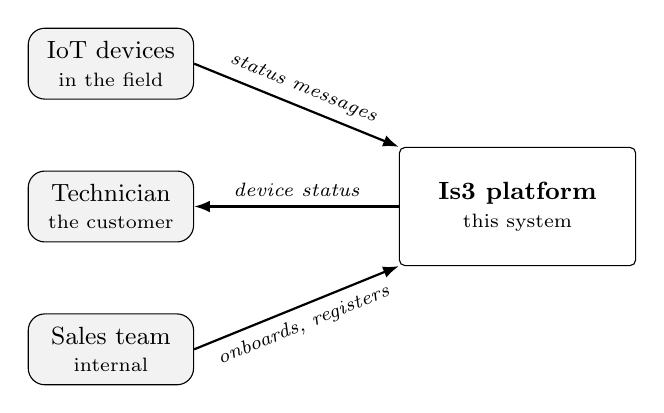
\begin{tikzpicture}[node distance=9mm and 26mm]
  \node[actor] (dev)  {IoT devices\\[-1pt]{\scriptsize in the field}};
  \node[actor, below=of dev] (tech) {Technician\\[-1pt]{\scriptsize the customer}};
  \node[actor, below=of tech] (sales) {Sales team\\[-1pt]{\scriptsize internal}};
  \node[box, right=of tech, minimum height=15mm, minimum width=30mm] (is3)
        {\textbf{Is3 platform}\\[-1pt]{\scriptsize this system}};
  \draw[ar] (dev.east)   -- (is3.north west) node[lbl, midway, above, sloped] {status messages};
  \draw[ar] (is3.west)   -- (tech.east)      node[lbl, midway, above] {device status};
  \draw[ar] (sales.east) -- (is3.south west) node[lbl, midway, below, sloped] {onboards, registers};
\end{tikzpicture}
\caption{Context. Note what is absent: no arrow runs from the technician to the
devices. There is no control path, by requirement.}
\end{figure}

\subsection*{C4 level 2 --- Containers}

\begin{figure}[H]
\centering
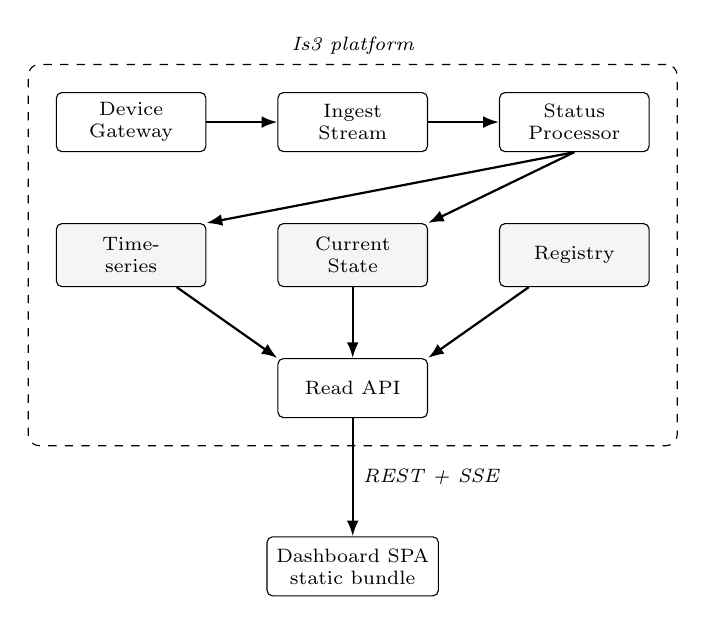
\begin{tikzpicture}[node distance=7mm and 9mm]
  \node[sml] (gw)   {Device\\Gateway};
  \node[sml, right=of gw] (str) {Ingest\\Stream};
  \node[sml, right=of str] (proc){Status\\Processor};
  \node[store, below=9mm of str]  (redis) {Current\\State};
  \node[store, left=of redis]     (ts)    {Time-\\series};
  \node[store, right=of redis]    (reg)   {Registry};
  \node[sml, below=9mm of redis]  (api)   {Read API};
  \node[sml, below=15mm of api]   (spa)   {Dashboard SPA\\{\scriptsize static bundle}};
  \draw[ar] (gw) -- (str);
  \draw[ar] (str) -- (proc);
  \draw[ar] (proc.south) -- (redis.north east);
  \draw[ar] (proc.south) -- (ts.north east);
  \draw[ar] (ts) -- (api.north west);
  \draw[ar] (redis) -- (api);
  \draw[ar] (reg) -- (api.north east);
  \draw[ar] (api) -- (spa) node[lbl, midway, right] {REST + SSE};
  \begin{scope}[on background layer]
    \node[env, fit=(gw)(str)(proc)(ts)(reg)(api),
          label={[font=\scriptsize\itshape]above:Is3 platform}] {};
  \end{scope}
\end{tikzpicture}
\caption{Containers. Arrows run one way throughout: with no user writes there is no
return path, so no distributed-transaction problem exists anywhere.}
\end{figure}

\subsection*{C4 level 3 --- Dashboard SPA}

\begin{figure}[H]
\centering
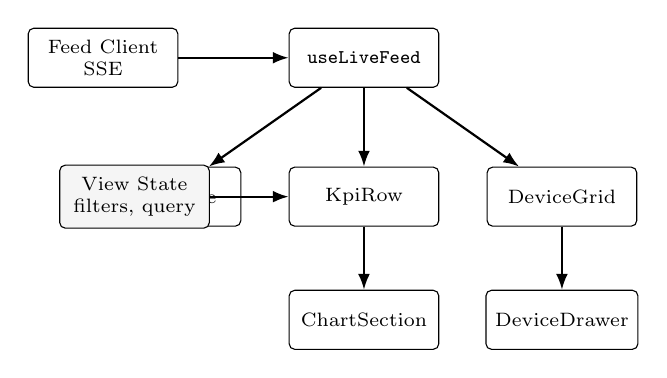
\begin{tikzpicture}[node distance=7mm and 8mm]
  \node[sml] (feed) {Feed Client\\{\scriptsize SSE}};
  \node[sml, right=14mm of feed] (hook) {\texttt{useLiveFeed}};
  \node[sml, below left=10mm and 6mm of hook] (pulse) {FleetPulse};
  \node[sml, below=10mm of hook] (kpi) {KpiRow};
  \node[sml, below right=10mm and 6mm of hook] (grid) {DeviceGrid};
  \node[sml, below=8mm of grid] (drawer) {DeviceDrawer};
  \node[sml, below=8mm of kpi]  (charts) {ChartSection};
  \node[store, left=10mm of kpi] (vs) {View State\\{\scriptsize filters, query}};
  \draw[ar] (feed) -- (hook);
  \draw[ar] (hook) -- (pulse);
  \draw[ar] (hook) -- (kpi);
  \draw[ar] (hook) -- (grid);
  \draw[ar] (grid) -- (drawer);
  \draw[ar] (kpi)  -- (charts);
  \draw[ar] (vs)   -- (kpi);
\end{tikzpicture}
\caption{The frontend. \texttt{useLiveFeed} is the seam: in production it wraps the
SSE connection, in this build it wraps a seeded generator. No component above it
changes when the source does.}
\end{figure}

\subsection*{Data flow --- one way, end to end}

\begin{figure}[H]
\centering
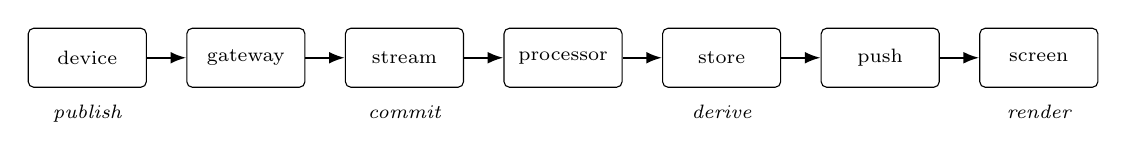
\begin{tikzpicture}[node distance=5mm]
  \node[sml, minimum width=15mm] (a) {device};
  \node[sml, minimum width=15mm, right=of a] (b) {gateway};
  \node[sml, minimum width=15mm, right=of b] (c) {stream};
  \node[sml, minimum width=15mm, right=of c] (d) {processor};
  \node[sml, minimum width=15mm, right=of d] (e) {store};
  \node[sml, minimum width=15mm, right=of e] (f) {push};
  \node[sml, minimum width=15mm, right=of f] (g) {screen};
  \foreach \s/\t/\ms in {a/b/200,b/c/100,c/d/300,d/e/{},e/f/{},f/g/200}
    {\draw[ar] (\s) -- (\t);}
  \node[lbl, below=1mm of a] {publish};
  \node[lbl, below=1mm of c] {commit};
  \node[lbl, below=1mm of e] {derive};
  \node[lbl, below=1mm of g] {render};
\end{tikzpicture}
\caption{A reading's journey. Budgeted against NFR-1: roughly 900\,ms of work inside
a 5\,s allowance, leaving headroom for network variance and retry.}
\end{figure}

\subsection*{How the architecture delivers each quality attribute}

\begin{center}
\small
\begin{tabularx}{\textwidth}{@{}l X@{}}
\toprule
\textbf{Attribute} & \textbf{Mechanism} \\
\midrule
Latency (NFR-1)          & Push over SSE, current state in memory, no polling \\
Read scalability (NFR-3/4) & Pre-aggregated rollups, cached responses, client-side filtering of an already-loaded fleet \\
Availability (NFR-5)     & Static client on a CDN; ingest decoupled by the stream, so it degrades alone \\
Durability (NFR-6)       & Durable partitioned stream with consumer offsets \\
Tenant isolation (NFR-8) & Tenant claim in the token, scope applied in the API, never in the client \\
Accessibility (NFR-10)   & Status as icon + label + colour; a table view on every chart \\
Portability (NFR-12)     & Static bundle with relative asset paths \\
\bottomrule
\end{tabularx}
\end{center}

%% ------------------------------------------------------- 3.5 the built system
\section{The built system (3.5)}

The architecture above was implemented and deployed. The frontend is a static bundle
published to GitHub Pages; the device feed is a seeded simulation behind
\texttt{useLiveFeed}, the same seam a real SSE client would occupy. The figures below
are screenshots of the running system, each tied to the requirement it satisfies.

\begin{figure}[htbp]
\centering
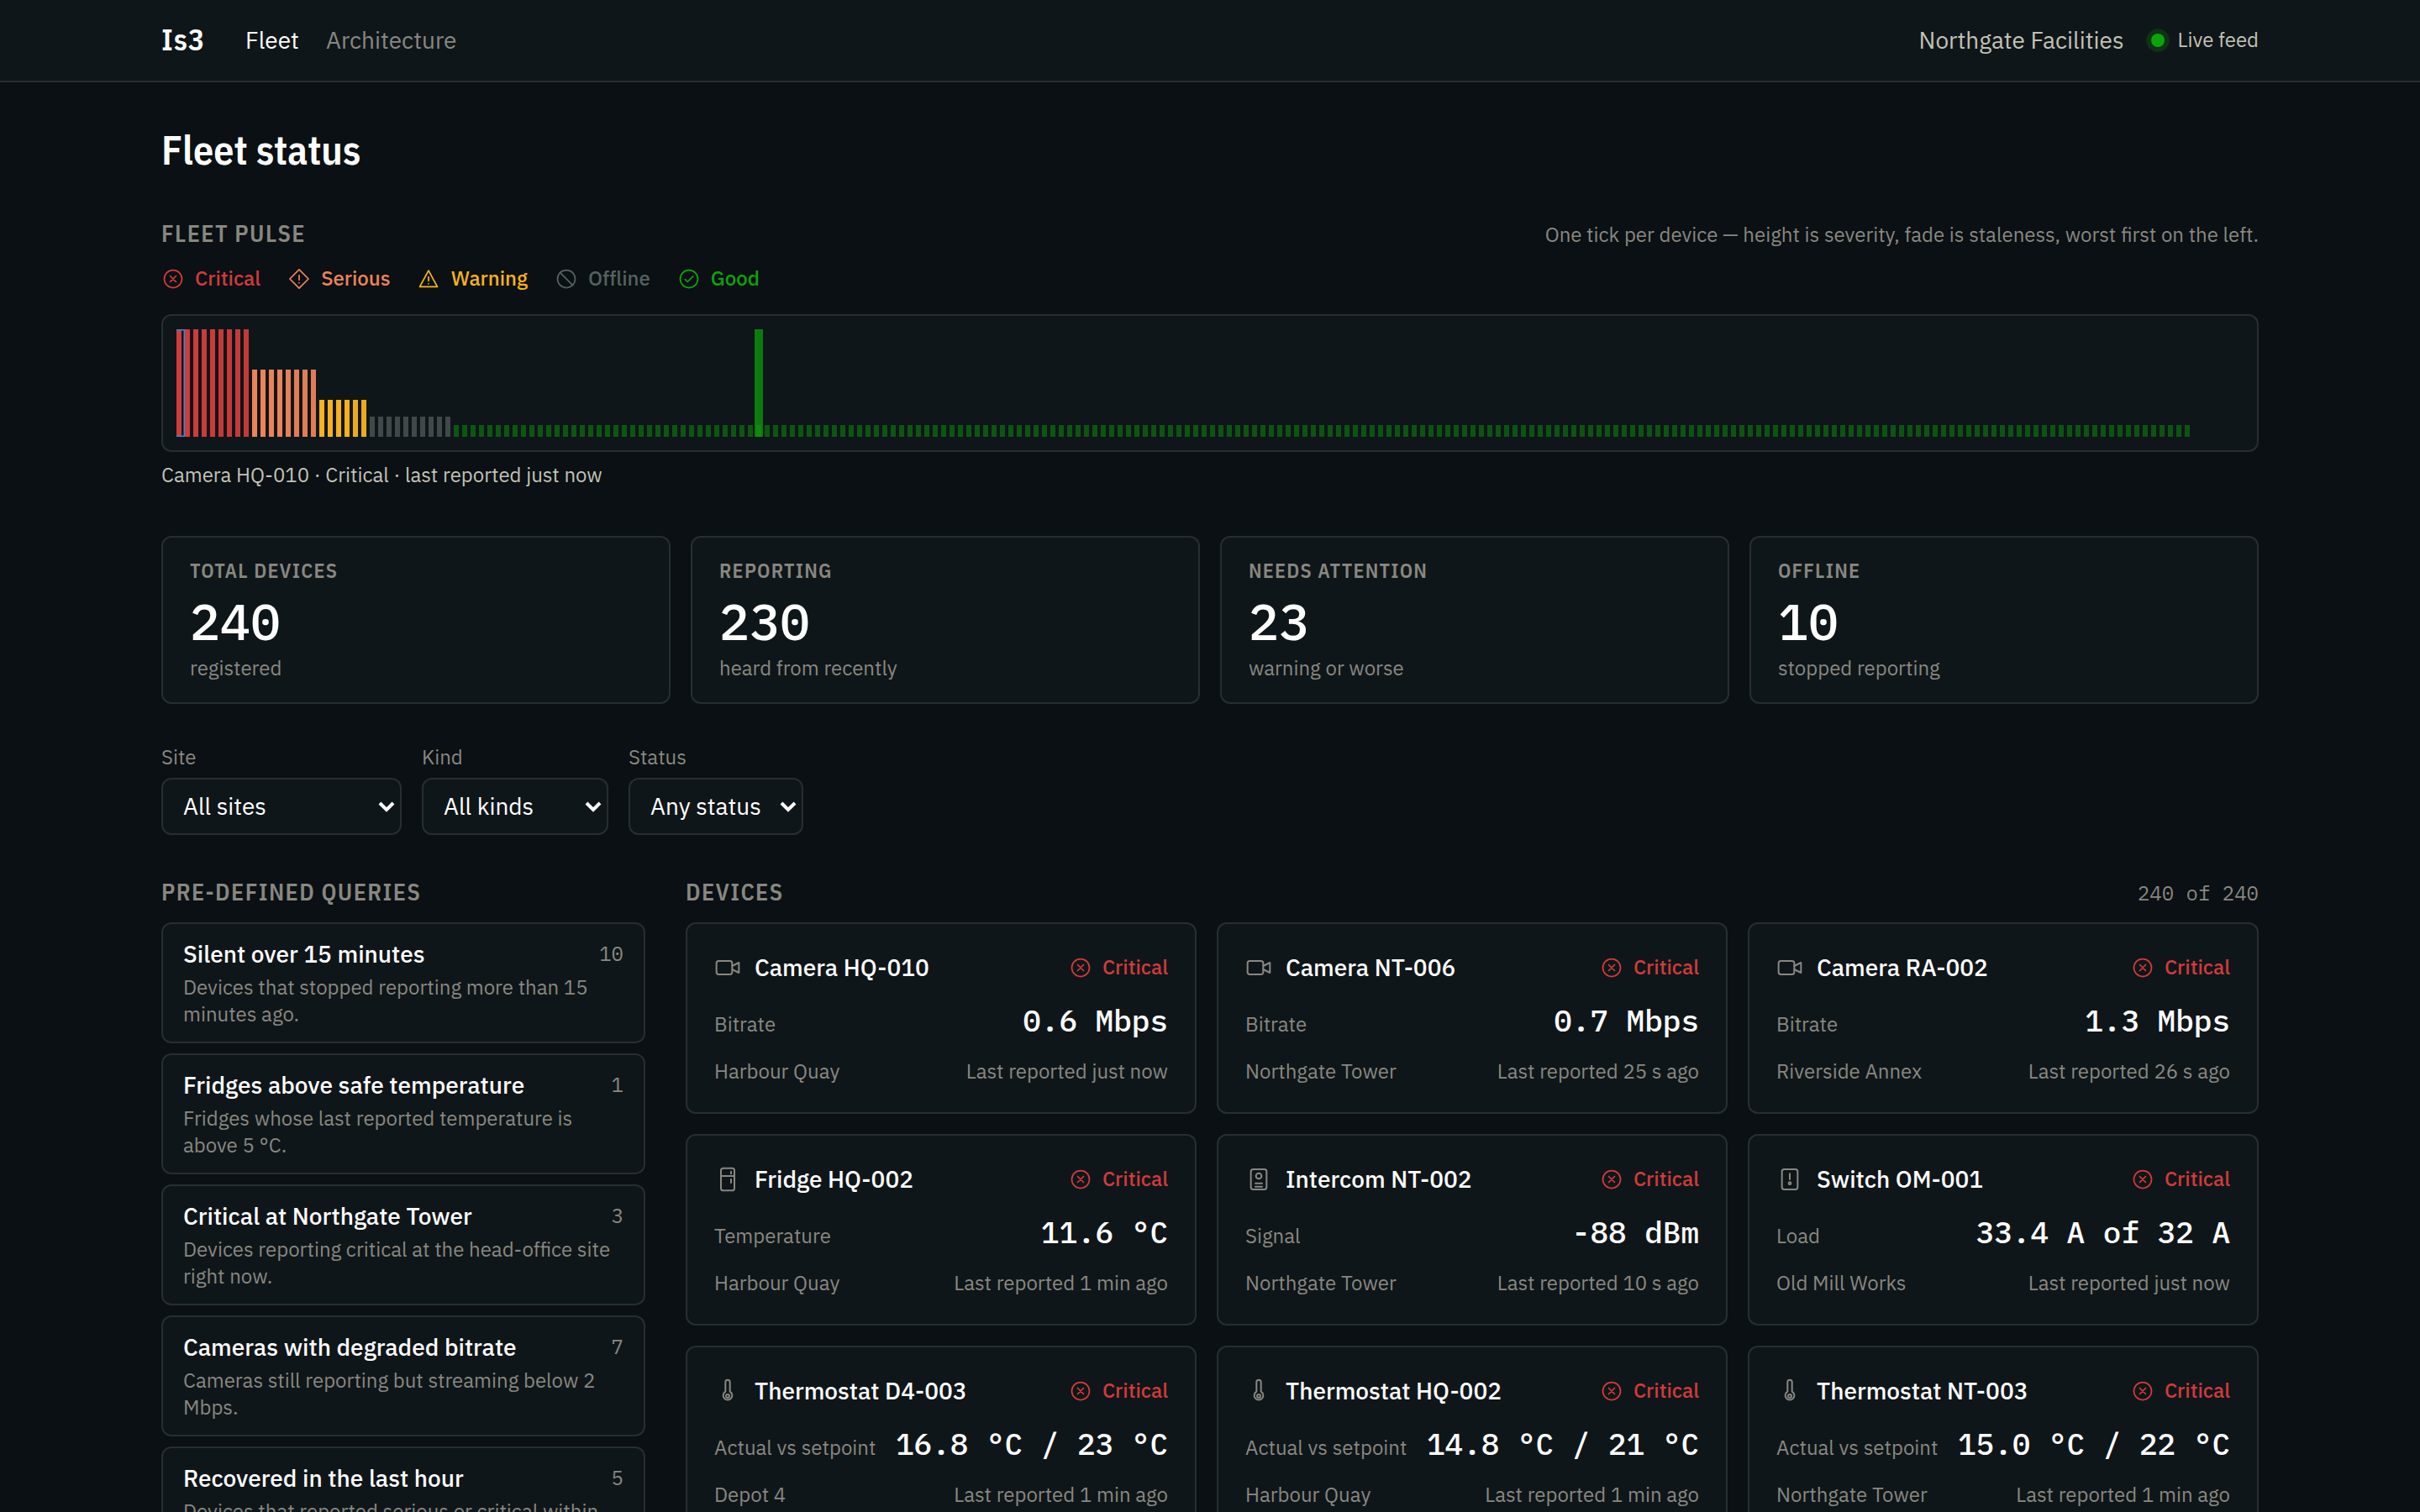
\includegraphics[width=\textwidth]{figures/fig-01-overview.png}
\caption{The whole fleet on one screen, each device showing status, kind, site and
last-seen time (FR-3, FR-4). The hero is the \emph{Fleet Pulse}: one tick per device,
height carrying severity and opacity carrying freshness, worst first.}
\end{figure}

\begin{figure}[htbp]
\centering
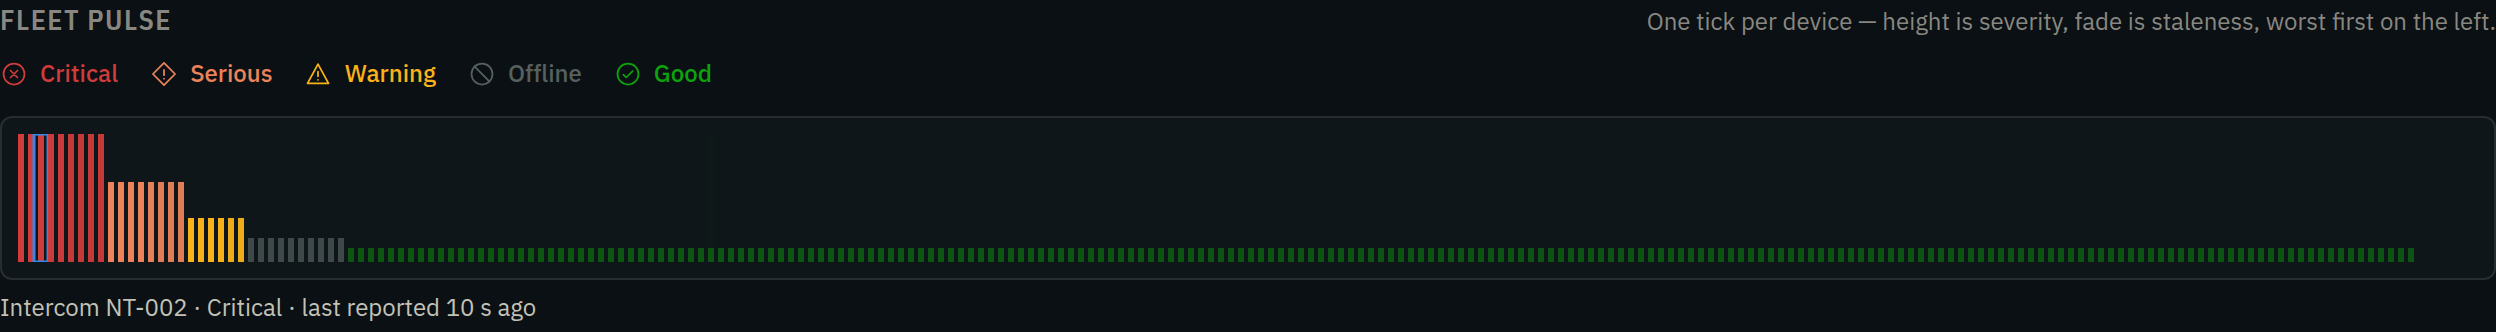
\includegraphics[width=\textwidth]{figures/fig-02-fleet-pulse.png}
\caption{Fleet Pulse in detail (FR-10, NFR-9). An earlier version encoded freshness as
height; since nearly every device is fresh nearly always, it rendered a uniform wall
of green and gave most of the visual weight to devices that are fine. Severity-driven
height inverts that, and double-encodes status as colour \emph{and} height.}
\end{figure}

\begin{figure}[htbp]
\centering
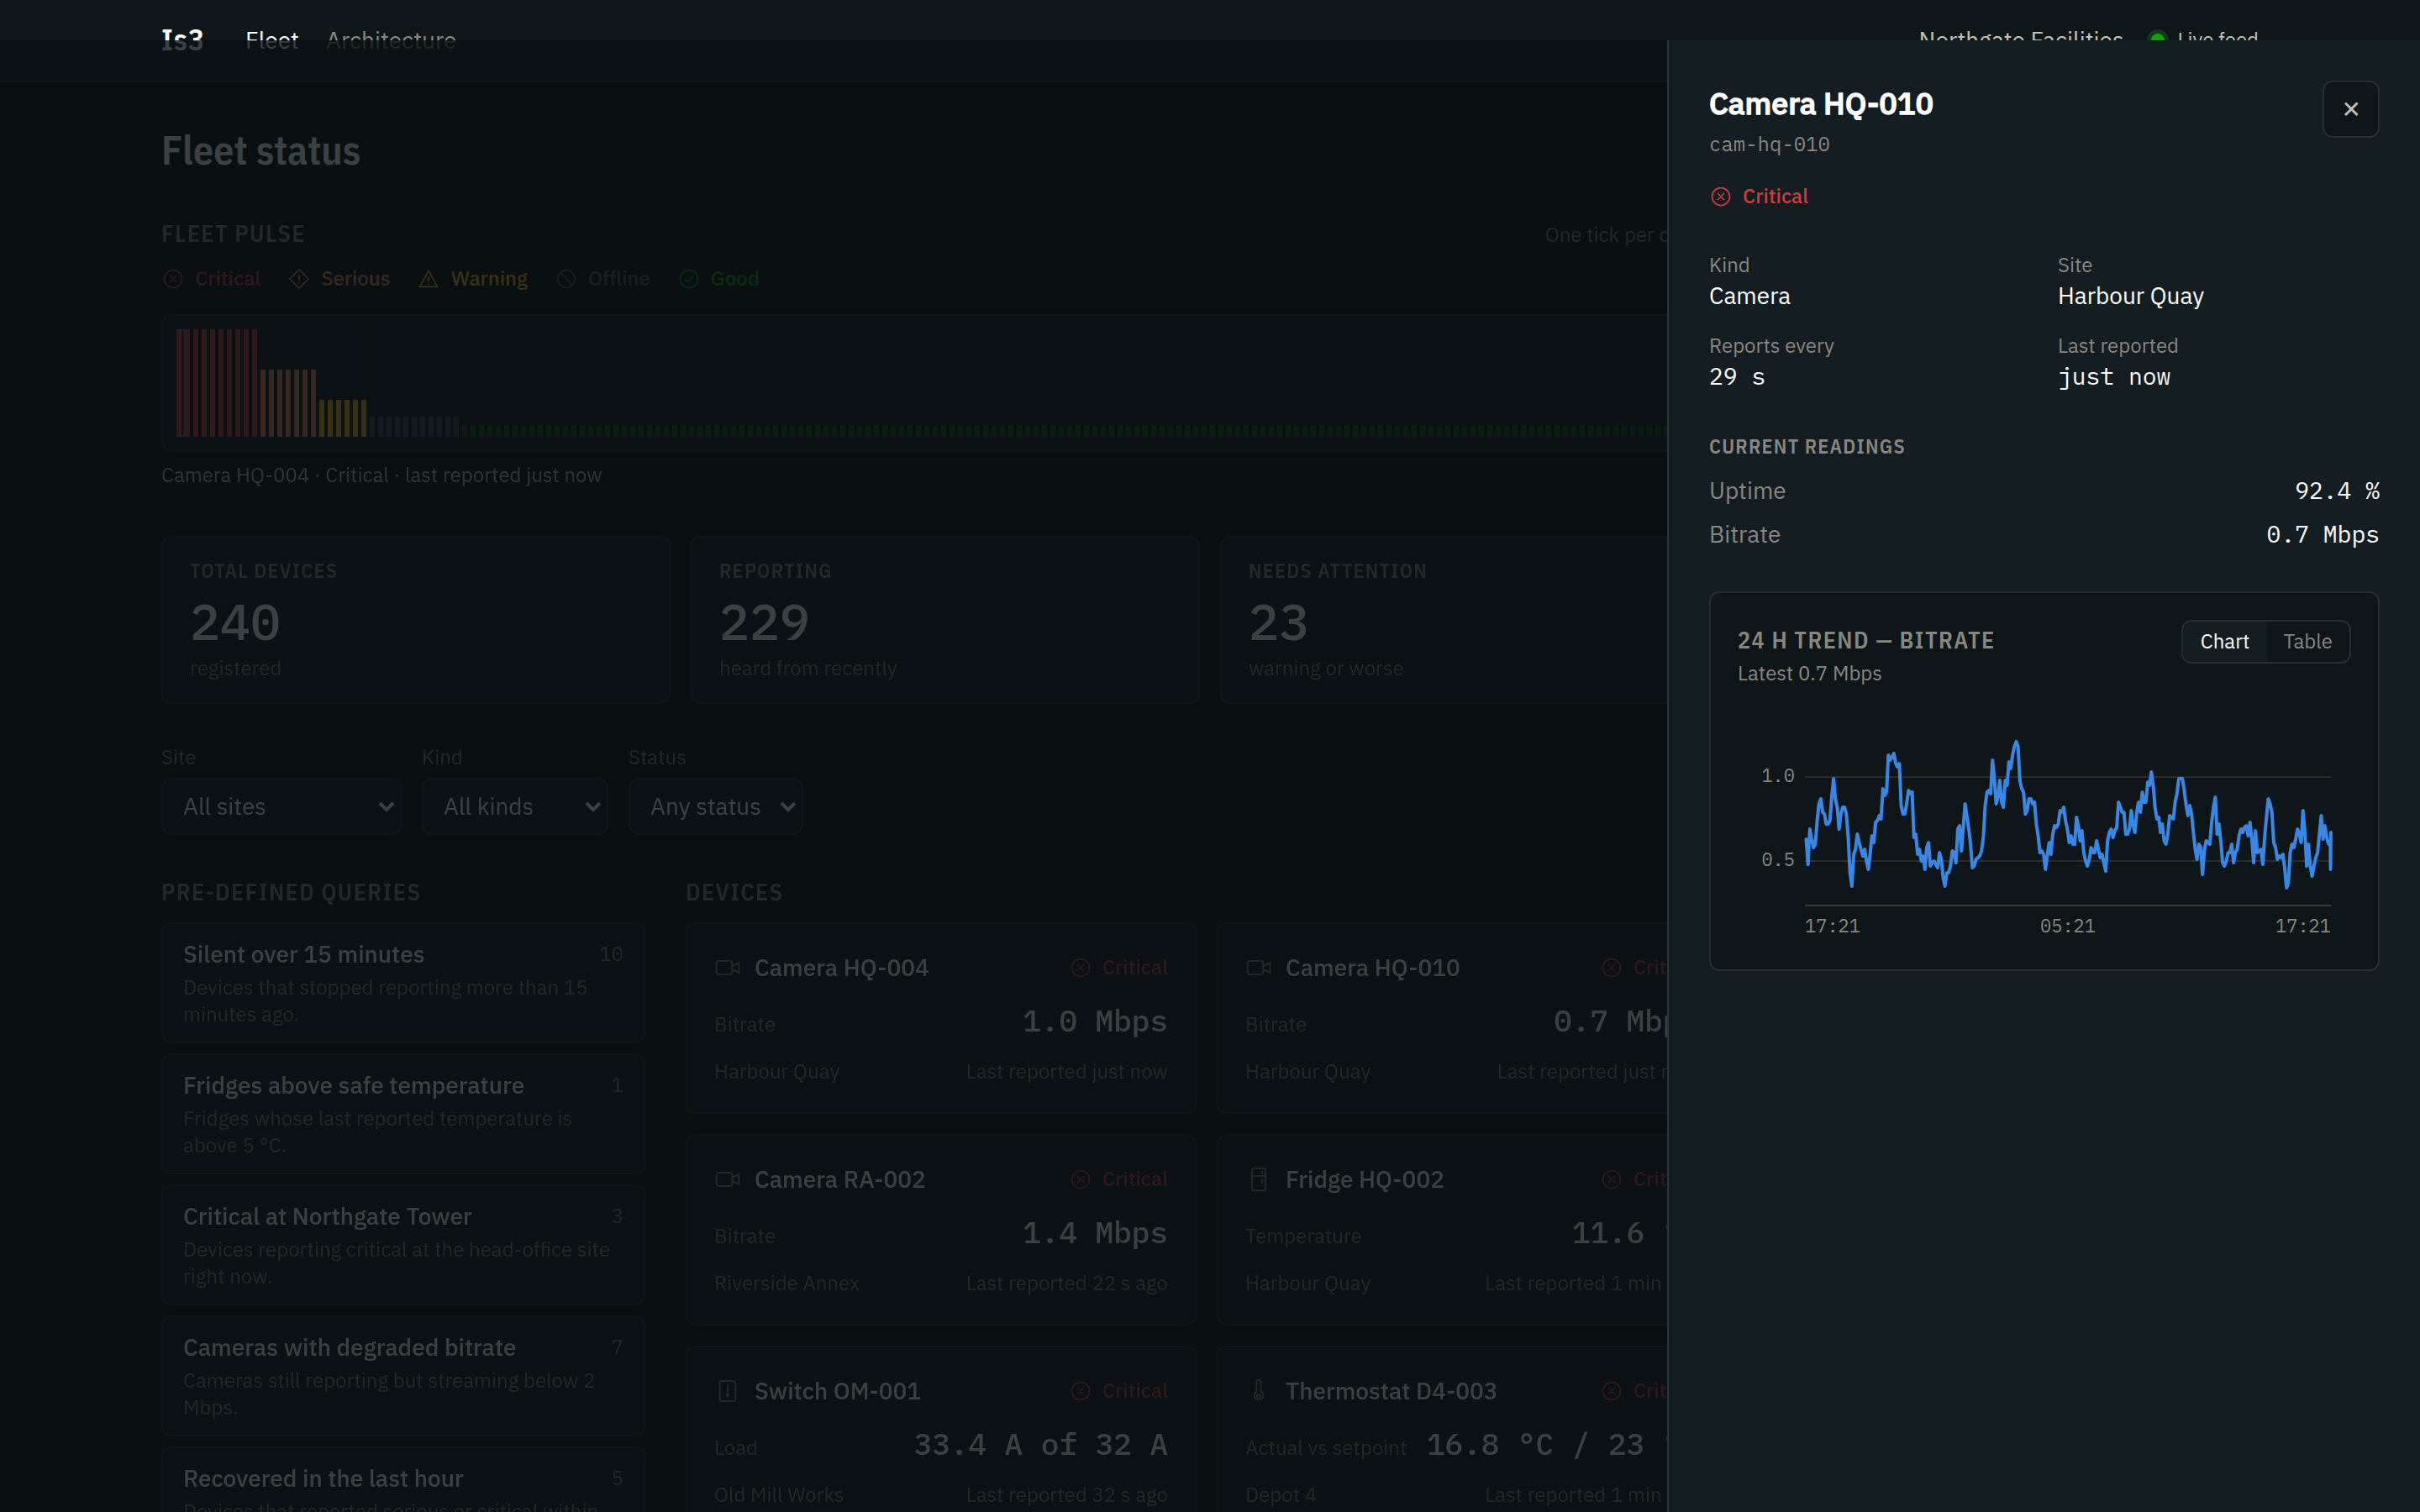
\includegraphics[width=\textwidth]{figures/fig-03-device-drawer.png}
\caption{A single device's recent history on demand (FR-9): identity, expected
reporting interval, current readings and a 24-hour trend with its own table view.}
\end{figure}

\begin{figure}[htbp]
\centering
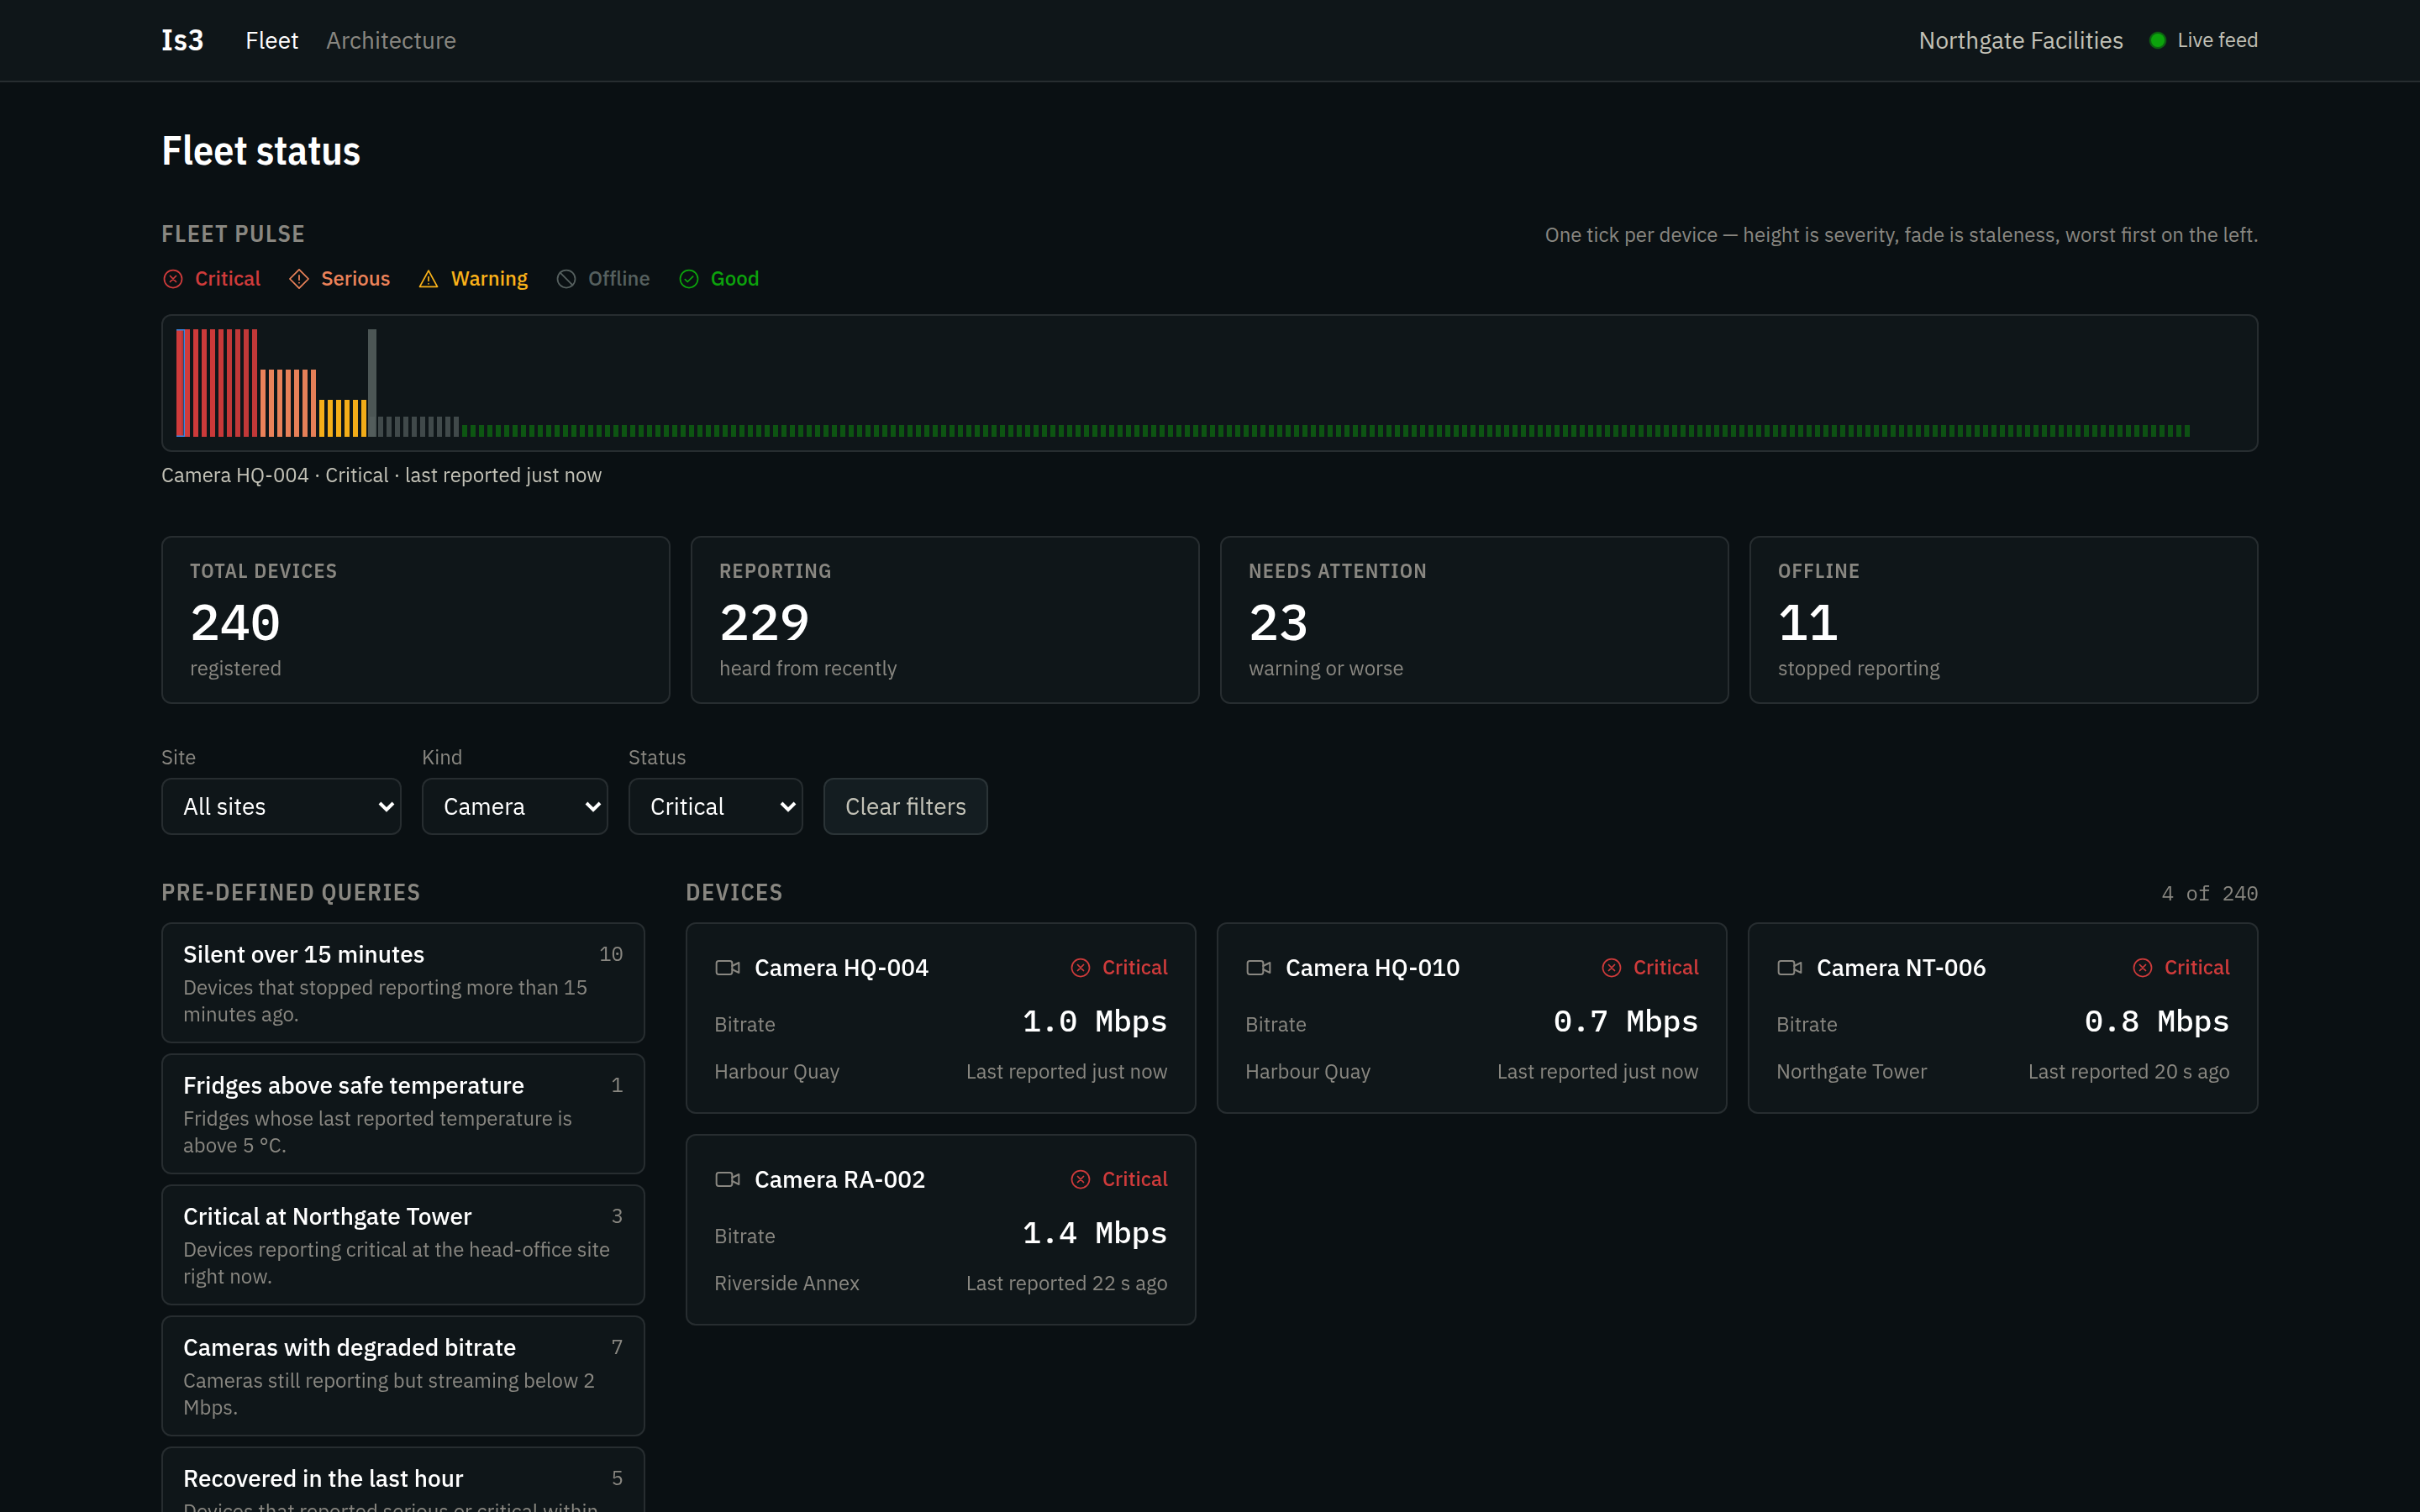
\includegraphics[width=\textwidth]{figures/fig-04-filters.png}
\caption{Composable filters (FR-8). Camera + Critical narrows 240 devices to 3.
Filtering is a pure function over the fleet already in the browser, so it costs no
round trip.}
\end{figure}

\begin{figure}[htbp]
\centering
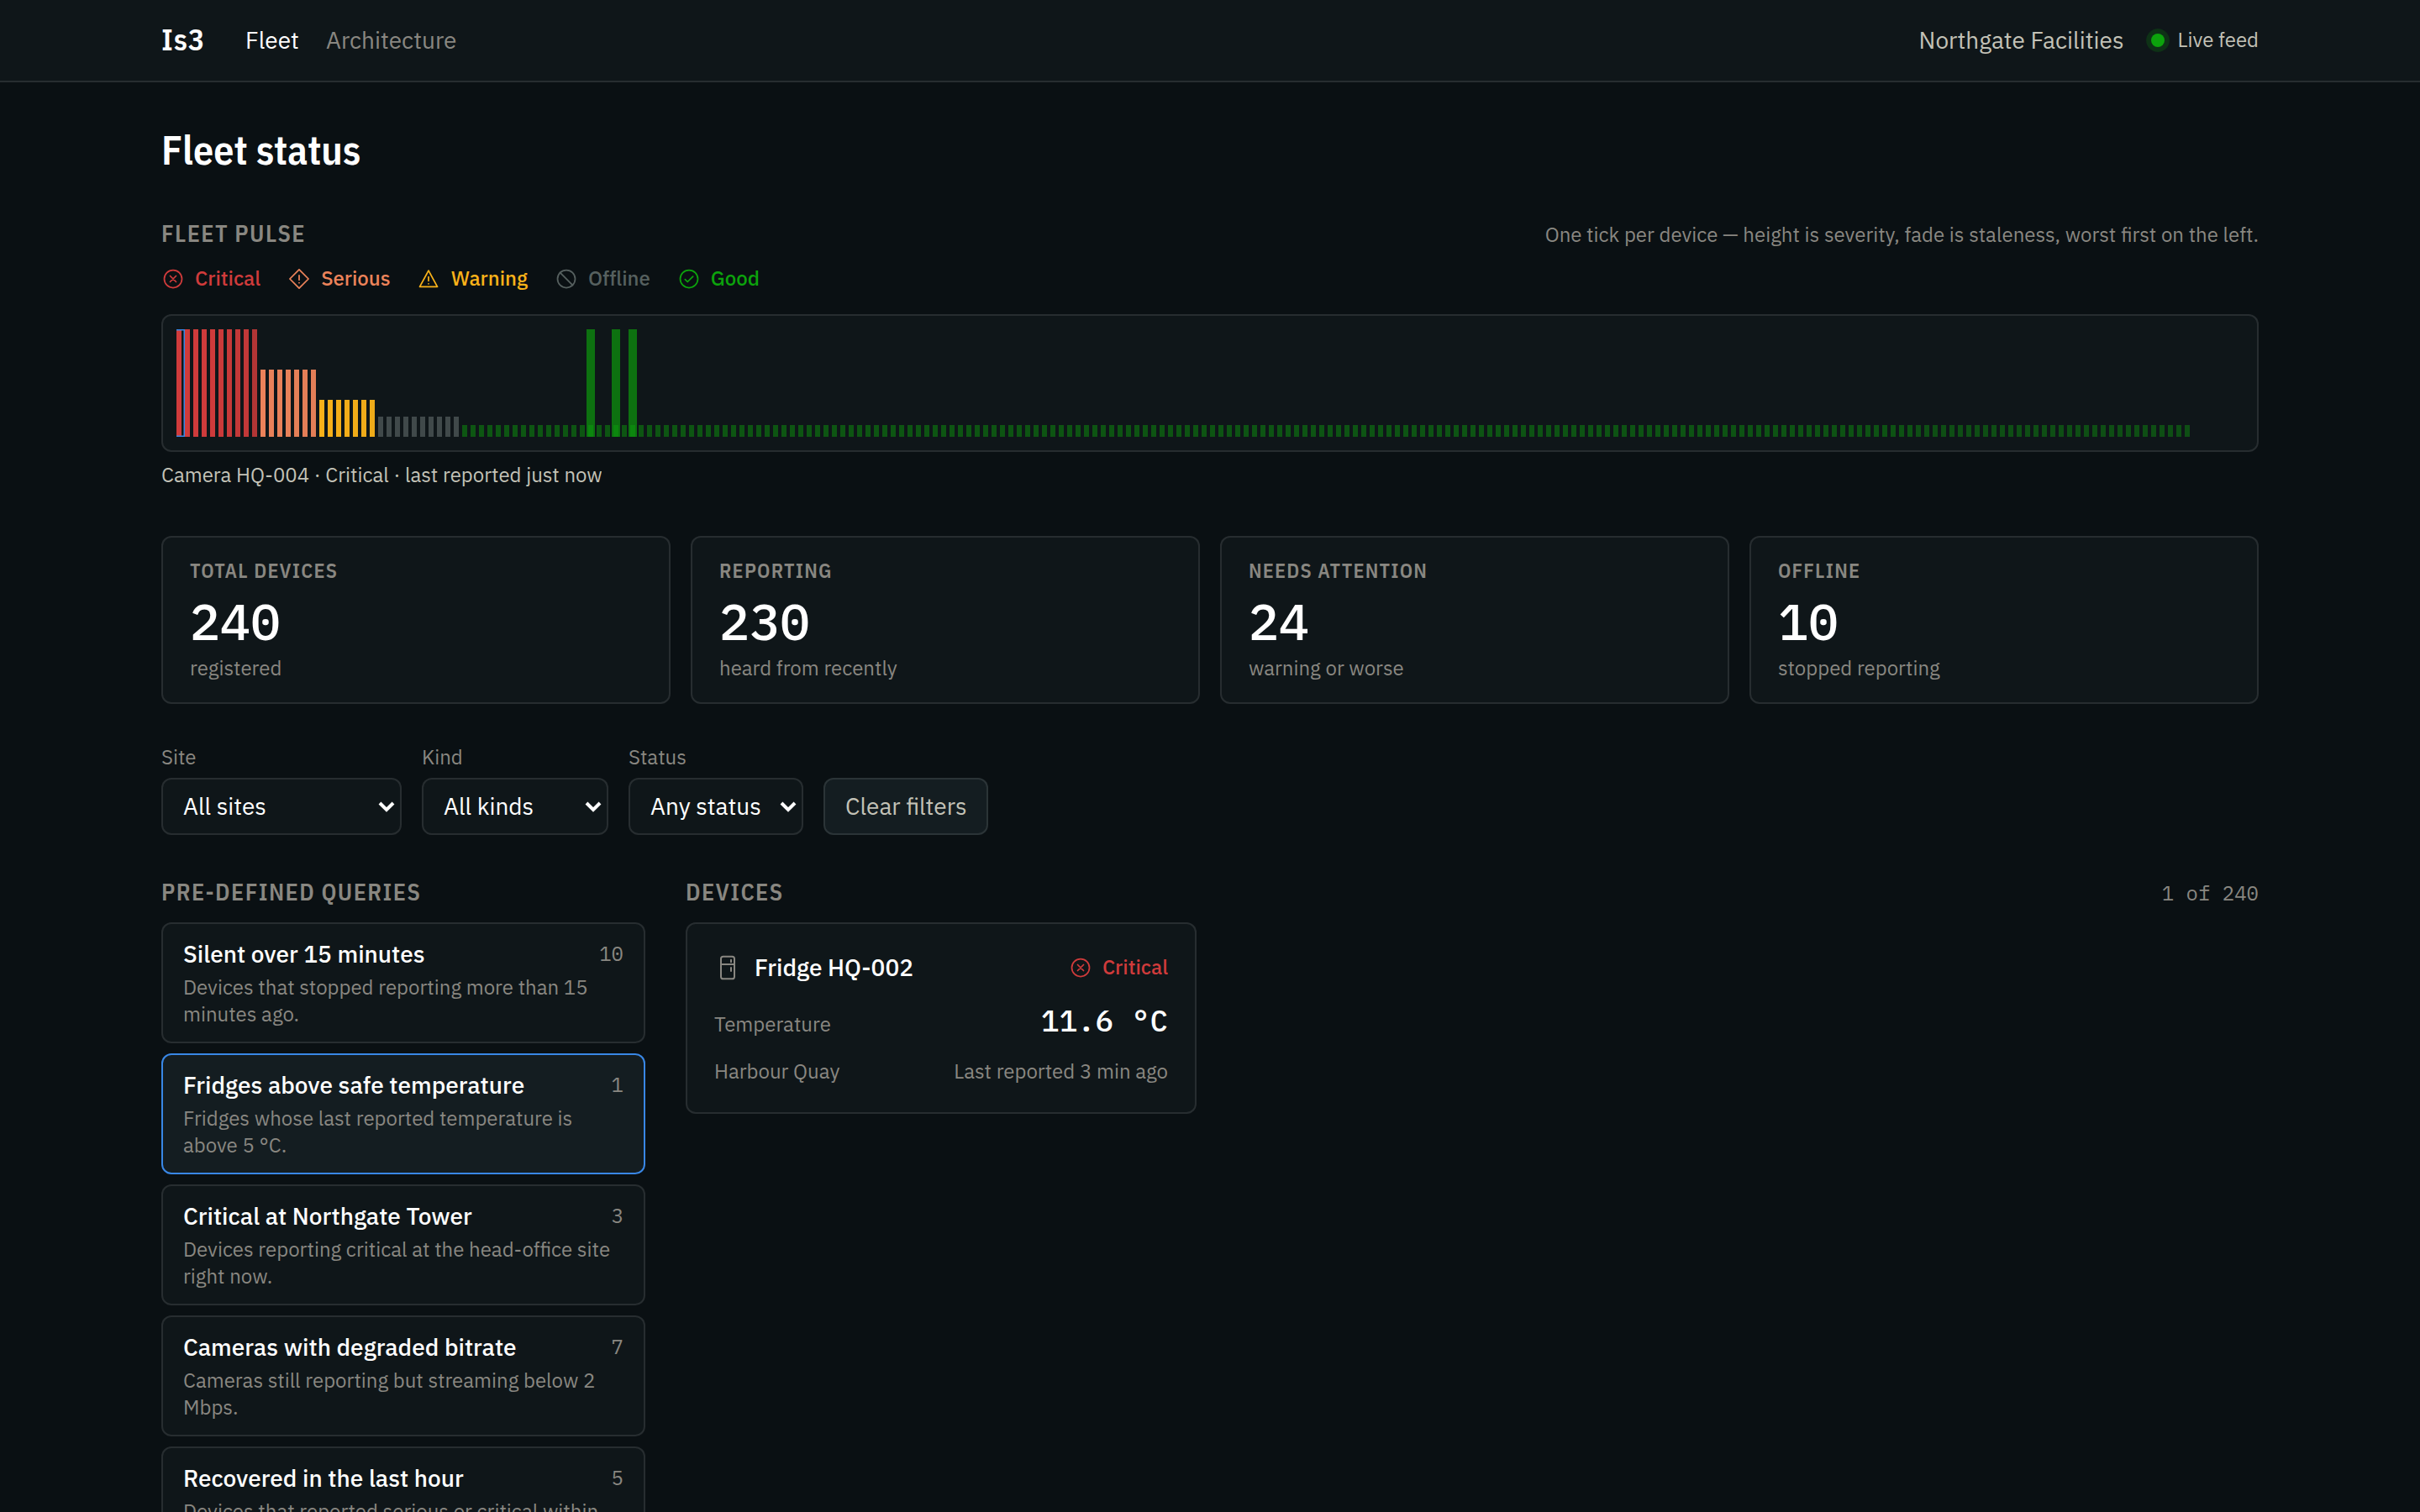
\includegraphics[width=\textwidth]{figures/fig-05-query.png}
\caption{A pre-defined query (FR-7). ``Fridges above safe temperature'' states a 5\,\textdegree C
threshold and returns one fridge reading 11.6\,\textdegree C. The customer picks an
identifier from a fixed catalogue; there is no free-form input anywhere on the page.}
\end{figure}

\begin{figure}[htbp]
\centering
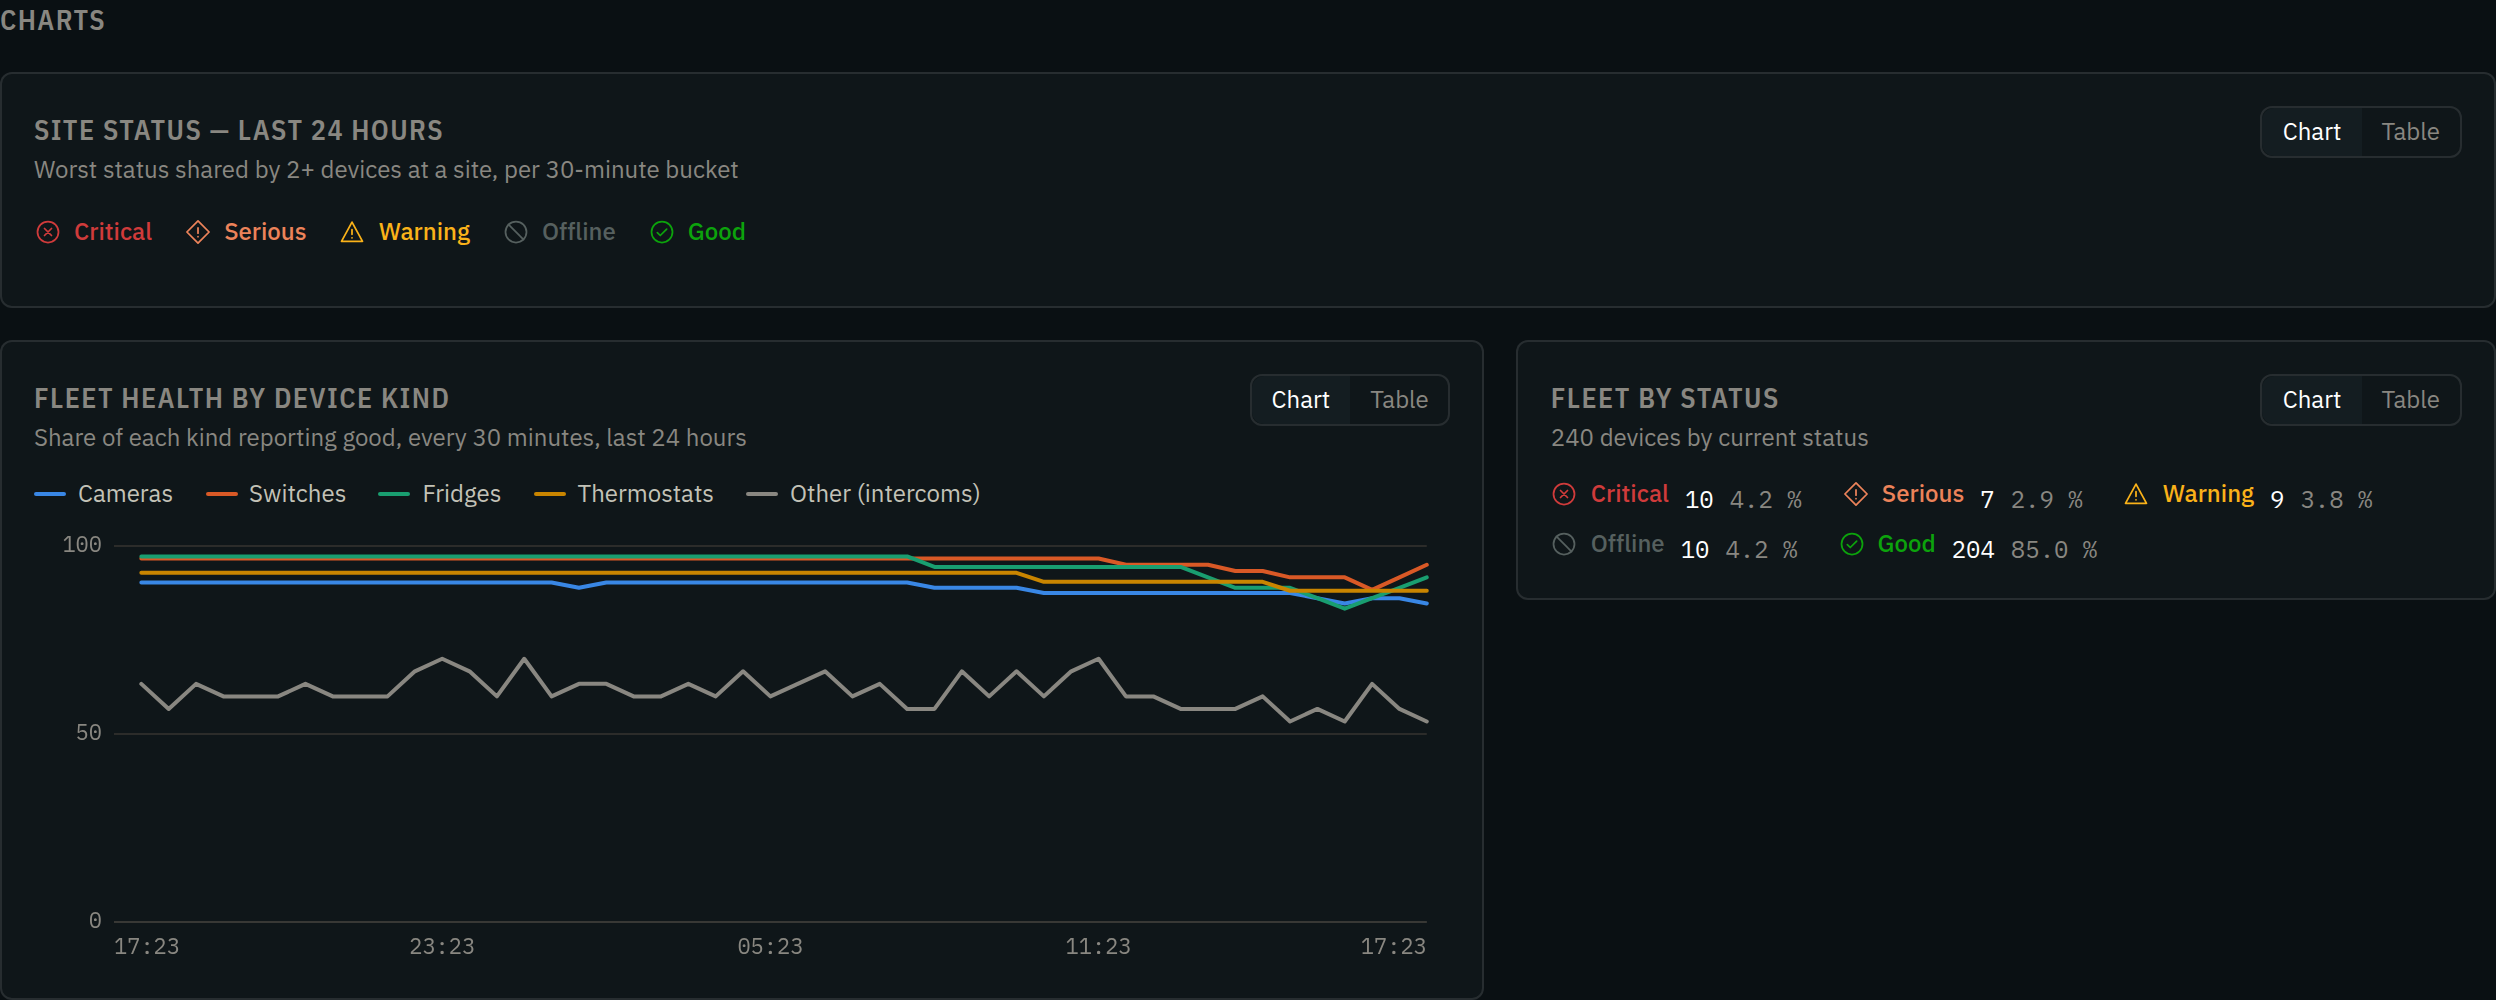
\includegraphics[width=\textwidth]{figures/fig-06-charts.png}
\caption{Fleet-level summaries (FR-10): site status over 24 hours, fleet health by
device kind, and composition by status. No chart has two y-axes, and series colours
follow the entity rather than its rank, so filtering never repaints the survivors.}
\end{figure}

\begin{figure}[htbp]
\centering
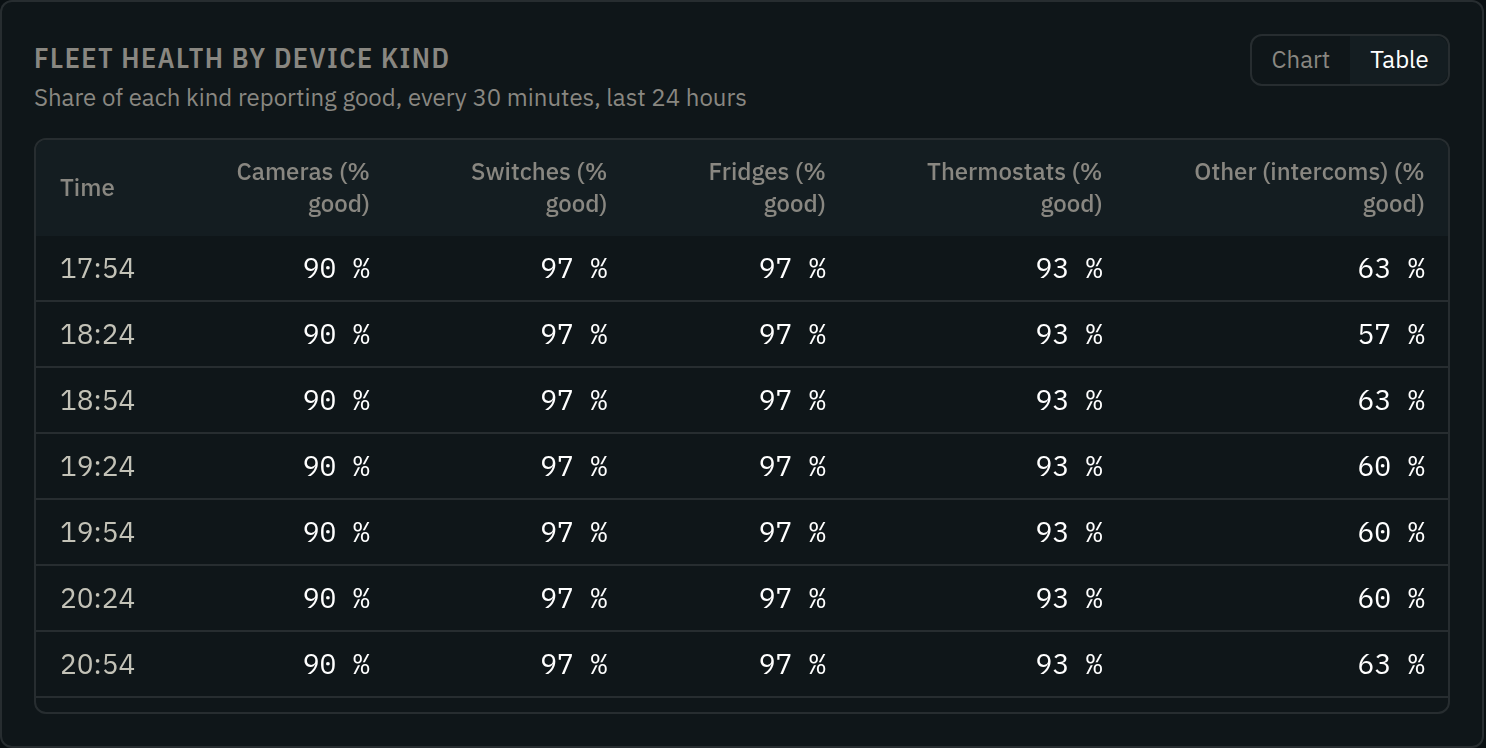
\includegraphics[width=0.86\textwidth]{figures/fig-07-table-view.png}
\caption{Every chart exposes the same numbers as a table (NFR-10). This is an
accessibility requirement, not a convenience: identity must never rest on colour
alone.}
\end{figure}

\begin{figure}[htbp]
\centering
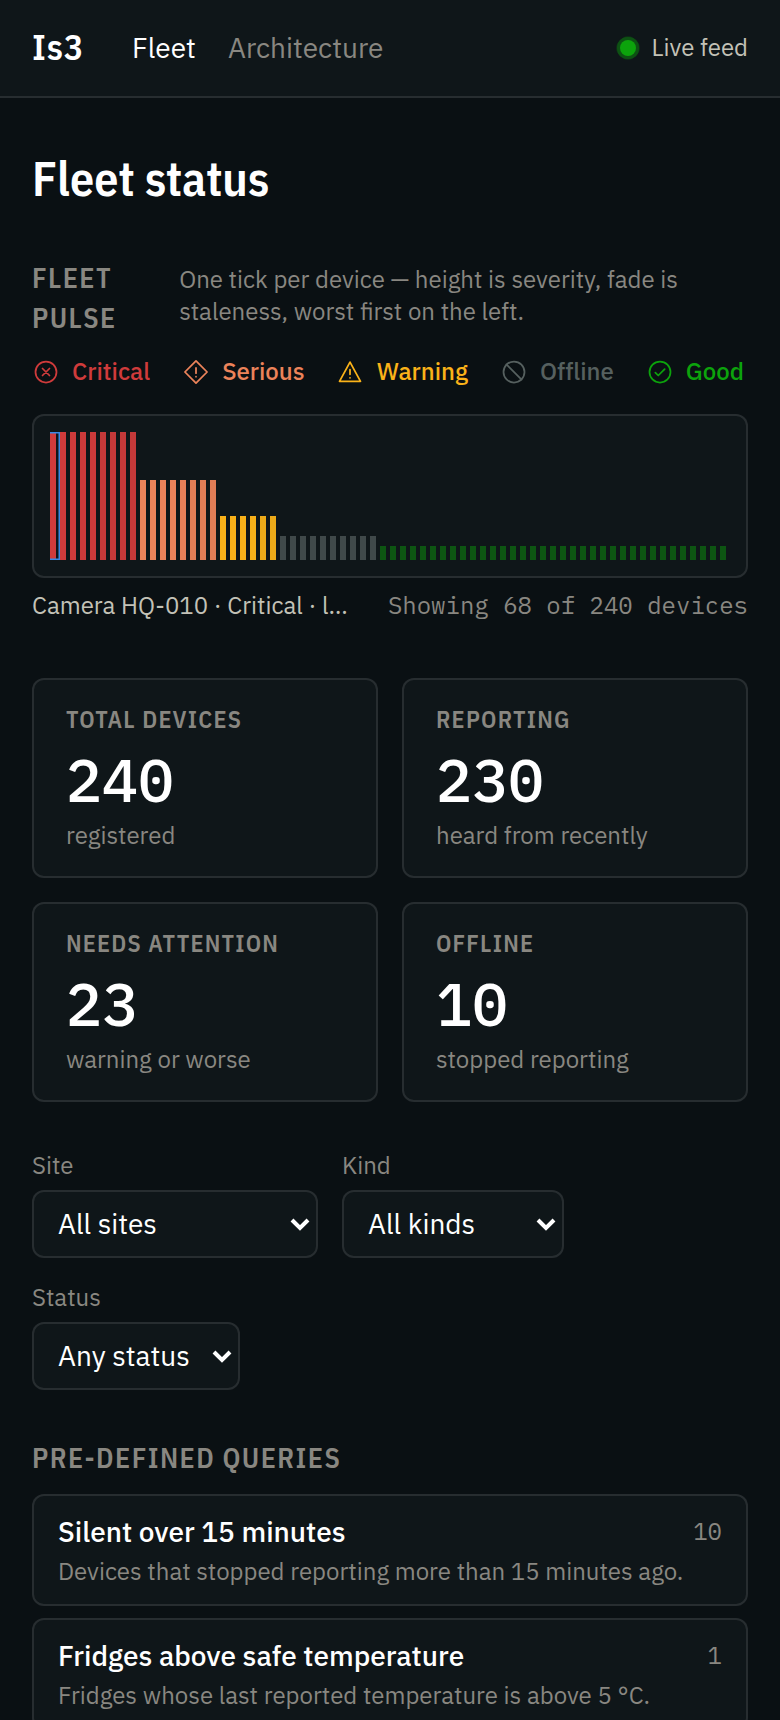
\includegraphics[width=0.42\textwidth]{figures/fig-08-mobile.png}
\hfill
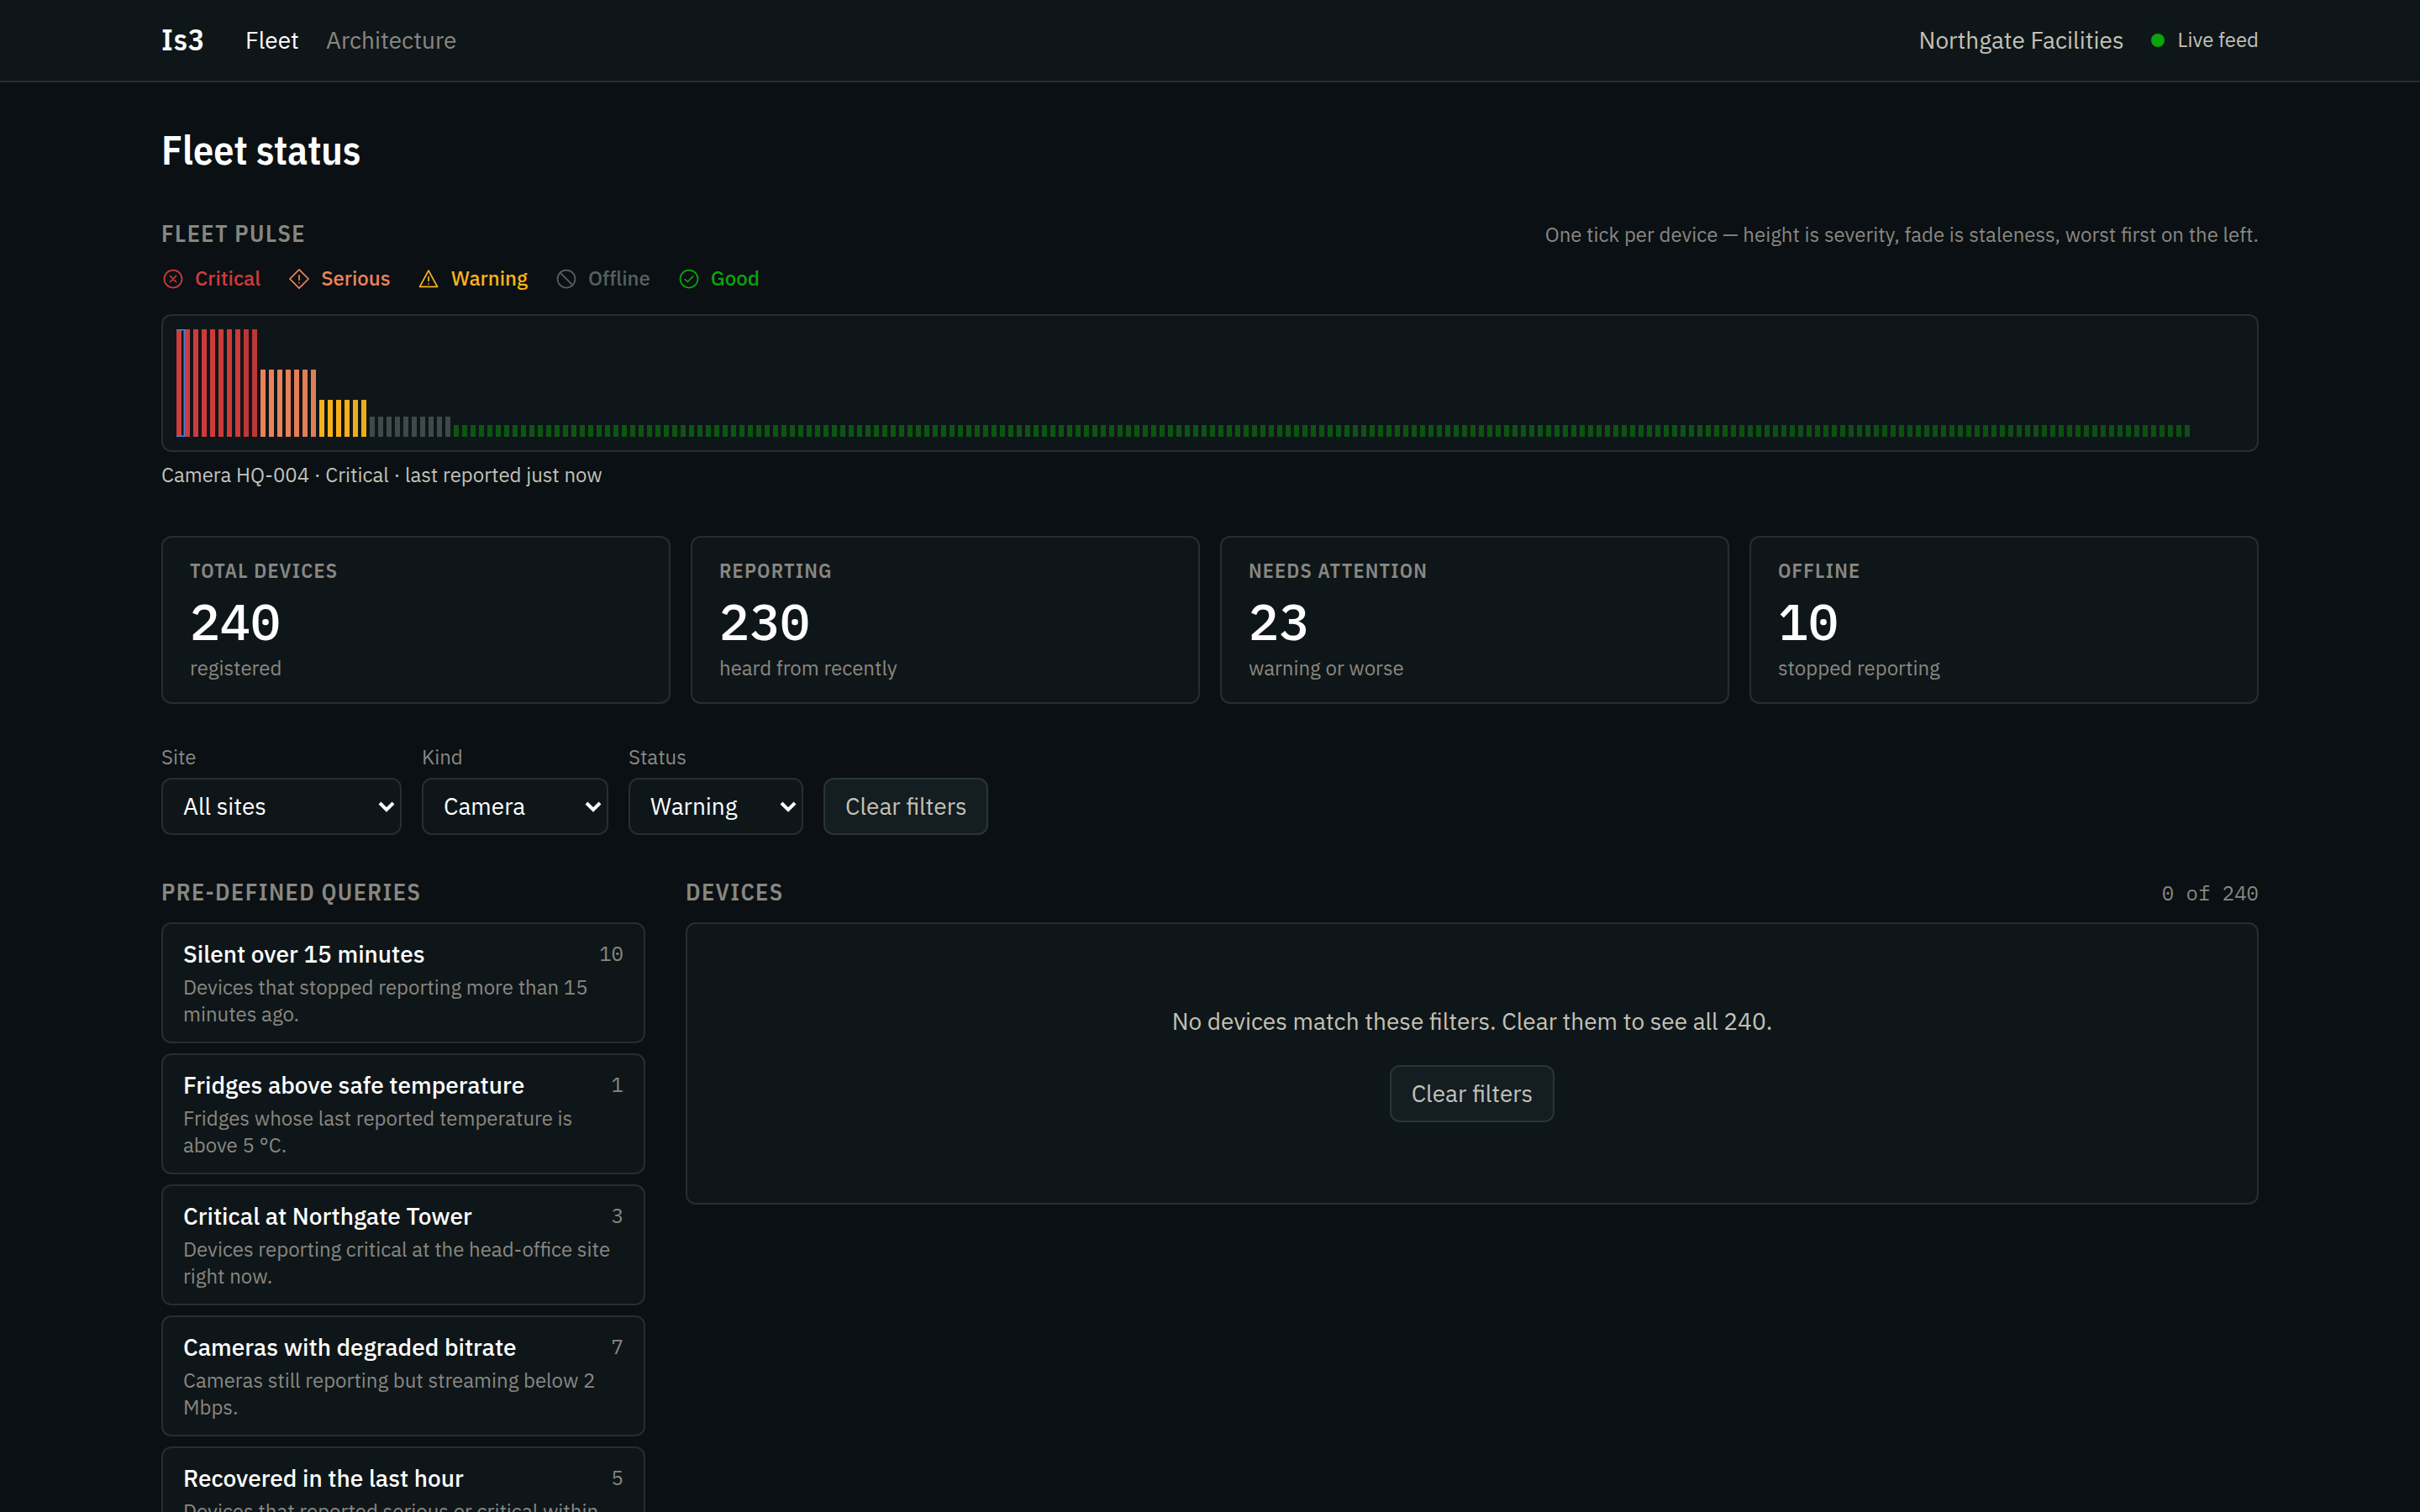
\includegraphics[width=0.52\textwidth]{figures/fig-09-empty-state.png}
\caption{Left: the layout at 390\,px; the Fleet Pulse reduces its tick count and says
so rather than squashing ticks illegibly. Right: an empty result is an invitation to
act, naming the number of devices a cleared filter would restore.}
\end{figure}

\clearpage

%% ------------------------------------------------------------------------ ADRs
\section{Architecture decision records}

\subsection*{ADR-001 --- Separate the ingest path from the read path}

\textbf{Context.} Devices push continuously and unpredictably; dashboards read a
small set repeatedly. The brief guarantees customers never write, removing the usual
reason to keep one model for both.

\textbf{Decision.} Devices publish into a durable partitioned stream. A processor
consumes it and maintains a small current-state store plus a time-series history. The
read API serves only from those stores and never touches the stream.

\textbf{Consequences.} Accepted: reads stay fast and cacheable regardless of ingest
load; processing can fail and catch up without loss; ingest degrades alone. Given up:
eventual consistency bounded by the 5\,s budget in NFR-1, one more system to operate,
and two stores holding overlapping data.

\subsection*{ADR-002 --- Pre-defined queries live server-side as a catalogue}

\textbf{Context.} FR-7 requires a fixed query set. The frontend is a static bundle, so
anything it holds is public.

\textbf{Decision.} Each query is a server-owned definition with an id, label,
description and parameterised implementation. The client sends
\texttt{\{queryId, params\}}; the server applies the tenant scope itself, always.

\textbf{Consequences.} Accepted: query cost is knowable and indexable in advance;
tenant scoping lives in one place; the client cannot express a query we did not plan
for --- which is the requirement, not a limitation. Given up: adding a query needs a
backend release, and power users cannot explore freely.

\subsection*{ADR-003 --- Charts are hand-built SVG, not a charting library}

\textbf{Context.} We committed to fixed-order series colours, no dual-axis charts, a
mandatory hover layer and a table view on every chart (NFR-10).

\textbf{Decision.} Small SVG components, one per chart form, sharing scale and axis
helpers. Series colours are keyed by entity identity, never by array index.

\textbf{Consequences.} Accepted: every rule is enforceable because we own the render
path; marks are real DOM nodes, so labels and focus come naturally; the chart layer
costs kilobytes rather than tens of kilobytes. Given up: we implement axes, ticks,
tooltips and legends ourselves, and a newcomer must learn our API rather than a
familiar one.

%% ----------------------------------------------------------------------- risks
\section{Known risks}

\begin{itemize}
  \item \textbf{The stream is the component whose loss hurts most.} Partitioning and
        replication mitigate it, but it remains a single conceptual point of failure.
  \item \textbf{Staleness detection depends on correct per-device expected
        intervals.} A wrong interval means either false offline alerts or silent dead
        devices. This needs to be a monitored data-quality metric, not a
        set-and-forget field.
  \item \textbf{Client-side filtering assumes the fleet fits in the browser.} True at
        10\,000 devices with a compact representation; beyond that, filtering moves
        server-side.
\end{itemize}

\end{document}
